\section{ĐỘNG HỌC NGHỊCH}
\subsection{Lập công thức giải bài toán động học nghịch}
Ta sẽ tính toán các công thức động học ngược robot từ bài toán động lực thuận.
\begin{center}
	\begin{tabular}{|m{2cm}|m{2cm}|m{2cm}|m{2cm}|m{2cm}|} 
		\hline
		Link & $a_{i}$ & $\alpha_{i}$ & $d_{i}$ & $\theta_{i}$\\ [0.5ex] 
		\hline
		1 & 0 & $\pi/2$ & $d_{1}$ & $\theta_{1}^{*}$\\ 
		\hline
		2 & $a_{2}$ & 0 & 0 & $\theta_{2}^{*}$\\
		\hline
		3 & $a_{3}$ & 0 & 0 & $\theta_{3}^{*}$\\ [0.5ex] 
		\hline
	\end{tabular}
\end{center}

\begin{center}
$^{0}T_{3} = {^{0}T_{1}} {^{1}T_{2}} {^{2}T_{3}} = \begin{bmatrix}
	c_{1}c_{23} & -c_{1}s_{23} & s_{1} & c_{1}(a_{2}c_{2}+a_{3}c_{23})\\
	s_{1}c_{23} & -s_{1}s_{23} & -c_{1} & s_{1}(a_{2}c_{2}+a_{3}c_{23})\\
	s_{23} & c_{23} & 0 & d_{1}+ a_{2}s_{2}+a_{3}s_{23}\\
	0 & 0 & 0 & 1
\end{bmatrix}$
\end{center}

Với input $

\subsection{Xây dựng UI và Animation cho bài toán động lực nghịch}
\subsubsection{Giao điện người dùng UI}

Xây dựng giao diện để người dùng nhập tọa độ vị trí của End effector, sau khi bấm nút \textit{Execute} robot sẽ tiến hành di chuyển đến vị trí trên.

\begin{figure}[H]
	\centering
	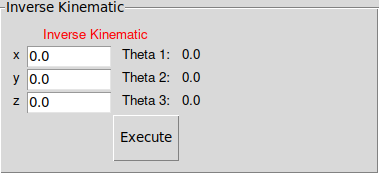
\includegraphics[width=1\linewidth]{Images/inv_ui.png}
	\caption{Giao diện Inverse Kinematic}
	\label{fig:enter-label8}
\end{figure}

\subsubsection{Tạo animation và di chuyển robot theo bài toán động lực nghịch}

Dựa vào các công thức đã lập được ở trên và các giá trị $x$, $y$ và $z$ do người dùng nhập ta tính ngược lại giá trị các góc $\theta_{1}$ , $\theta_{2}$ và $\theta_{3}$, sau khi kiểm tra các góc xaoy có nằm trong phạm vi giới hạn quya của từng khớp ta tiến hành cho robot chuyển động giống như bài toán thuận theo các giá trị $\theta$ vừa tính được ở trên.

\vspace{0.5cm}
\begin{lstlisting}[language=python]
	def inverseKine():
	global guiThetaInv
	px = guiCoorInv[0].get()
	py = guiCoorInv[1].get()
	pz = guiCoorInv[2].get()-d[0]
	# Check valid
	valid = 0
	tmp = (px**2+py**2+pz**2)**0.5
	if (tmp <= a[1]+a[2]) and (tmp >= abs(a[1]-a[2])) and (pz+d[0] >= 0): 
	# calculate
	c3 = (px**2+py**2+pz**2-a[1]**2-a[2]**2)/(2*a[1]*a[2])
	s3 = (1-c3**2)**0.5
	theta3 = atan2(s3, c3)
	
	theta2 = atan2(pz, (px**2+py**2)**0.5) - acos((px**2+py**2+pz**2+a[1]**2-a[2]**2)/(2*a[1]*(px**2+py**2+pz**2)**0.5))
	
	theta1 = atan2(py, px)
	
	valid = 1
	for i, thetaN in enumerate([theta1, theta2, theta3]):
	if thetaN < limitTheta[i][0] or thetaN > limitTheta[i][1]:
	valid = 0
	else: guiThetaInv[i].set(round(thetaN*180/pi, 3))
	
	if valid:
	deltaTime = 60
	nextTheta = np.array([theta1, theta2, theta3])
	stepAngle = np.array([(nextTheta[0]-theta[0])/deltaTime, (nextTheta[1]-theta[1])/deltaTime, (nextTheta[2]-theta[2])/deltaTime])
	animateTranform(nextTheta, stepAngle, deltaTime)
	else:
	tkinter.messagebox.showwarning("Inverse Kinematic.",  "Out of workspace")
\end{lstlisting}

\begin{figure}[H]
	\centering
	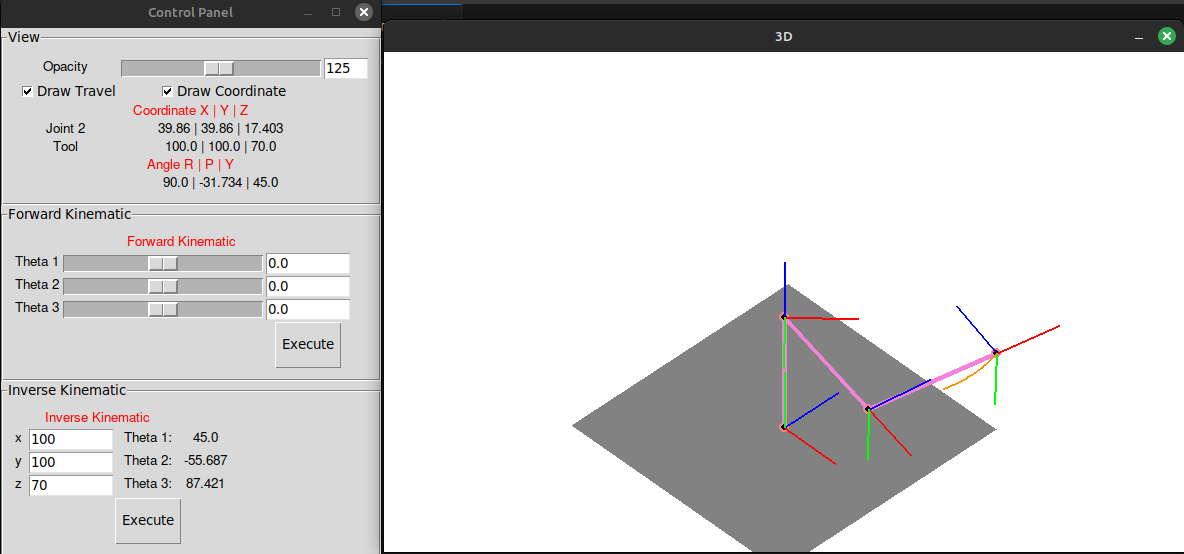
\includegraphics[width=1\linewidth]{Images/inv_demo.png}
	\caption{Inverse Kinematic}
	\label{fig:enter-label9}
\end{figure}